\documentclass{article}
% translate with >> pdflatex -shell-escape <file>

% This file is an extract of the PGFPLOTS manual, copyright by Christian Feuersaenger.
% 
% Feel free to use it as long as you cite the pgfplots manual properly.
%
% See
%   http://pgfplots.sourceforge.net/pgfplots.pdf
% for the complete manual.
%
% Any required input files (for <plot table> or <plot file> or the table package) can be downloaded
% at
% http://www.ctan.org/tex-archive/graphics/pgf/contrib/pgfplots/doc/latex/
% and
% http://www.ctan.org/tex-archive/graphics/pgf/contrib/pgfplots/doc/latex/plotdata/

\usepackage{pgfplots}
\pgfplotsset{compat=newest}

\pagestyle{empty}

\begin{document}
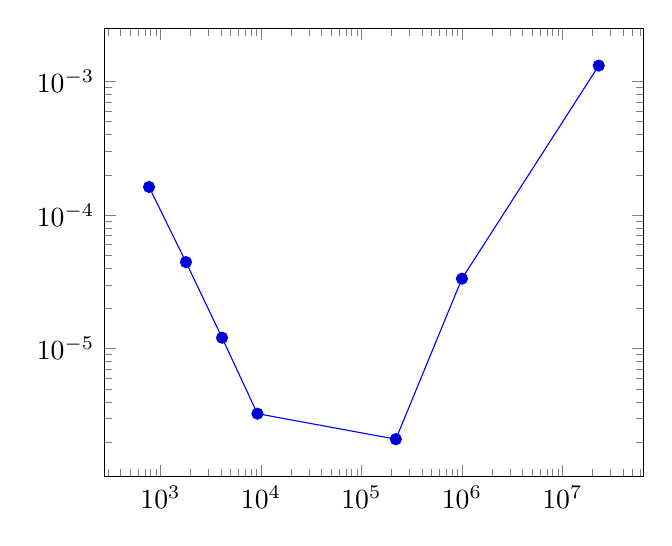
\begin{tikzpicture}
\begin{loglogaxis}
\addplot coordinates {
	(769,   1.6227e-04)
	(1793,  4.4425e-05)
	(4097,  1.2071e-05)
	(9217,  3.2610e-06)
	(2.2e5, 2.1E-6)
	(1e6,   0.00003341)
	(2.3e7, 0.00131415)
};
\end{loglogaxis}
\end{tikzpicture}
\end{document}
